\section*{Consulta 2: Cantidad de asistentes y ganancias por disciplina y localidad}

\subsection*{Descripción}
Esta consulta calcula cuántas personas asistieron y cuánto dinero se ganó en cada disciplina y localidad. Es útil para evaluar el éxito financiero y la popularidad de los eventos en distintas áreas.

\textbf{SQL}

\begin{verbatim}
SELECT 
    d.NombreDisciplina,
    l.NombreLocalidad,
    SUM(e.Precio) AS GananciasTotales,
    COUNT(ce.IDCliente) AS CantidadAsistentes
FROM 
    Evento e
JOIN 
    Disciplina d ON e.IDDisciplina = d.IDDisciplina
JOIN 
    Localidad l ON e.NombreLocalidad = l.NombreLocalidad AND e.IDDisciplina = l.IDDisciplina
JOIN 
    CompraEntrada ce ON e.IDEvento = ce.IDEvento
GROUP BY 
    d.NombreDisciplina, l.NombreLocalidad
ORDER BY 
    CantidadAsistentes DESC;
\end{verbatim}

\begin{center}
    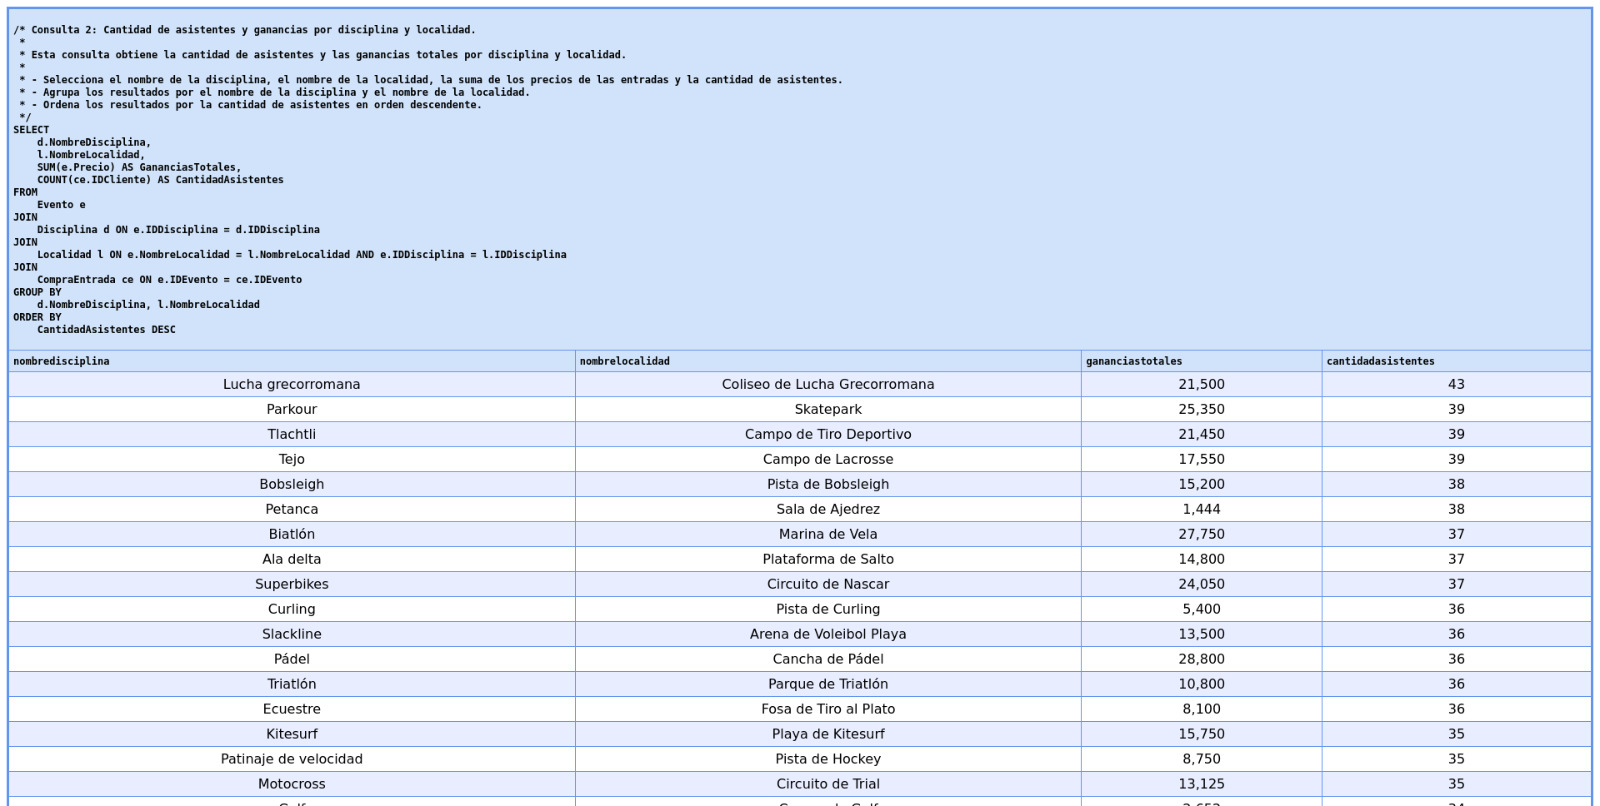
\includegraphics[width=16.5cm]{../resources/Chapters/Consultas/Imagenes/Consulta2.jpeg} 
    
   Consulta 2. Cantidad de asistentes y ganancias por disciplina y localidad. 
\end{center}

\textbf{Desglose de la consulta}

\begin{itemize}
   \item \textbf{Selección de columnas (\texttt{SELECT})}:
   \begin{itemize}
       \item Se seleccionan las siguientes columnas:
       \begin{itemize}
           \item \texttt{d.NombreDisciplina}: Nombre de la disciplina.
           \item \texttt{l.NombreLocalidad}: Nombre de la localidad.
           \item \texttt{SUM(e.Precio)}: Suma de los precios de las entradas, denominada \texttt{GananciasTotales}.
           \item \texttt{COUNT(ce.IDCliente)}: Cuenta la cantidad de asistentes, denominada \texttt{CantidadAsistentes}.
       \end{itemize}
   \end{itemize}
   
   \item \textbf{Tablas involucradas (\texttt{FROM} y \texttt{JOIN})}:
   \begin{itemize}
       \item La consulta utiliza cuatro tablas:
       \begin{itemize}
           \item \texttt{Evento (e)}: Contiene la información de los eventos.
           \item \texttt{Disciplina (d)}: Contiene la información de las disciplinas.
           \item \texttt{Localidad (l)}: Contiene la información de las localidades.
           \item \texttt{CompraEntrada (ce)}: Contiene la información de las entradas compradas.
       \end{itemize}
       \item Se realizan \texttt{JOINs} entre las tablas para relacionar los eventos con las disciplinas, localidades y entradas compradas.
   \end{itemize}
   
   \item \textbf{Agrupación de resultados (\texttt{GROUP BY})}:
   \begin{itemize}
       \item Para calcular la cantidad de asistentes y las ganancias por disciplina y localidad, se agrupan los datos según las columnas:
       \begin{itemize}
           \item \texttt{d.NombreDisciplina}, \texttt{l.NombreLocalidad}.
       \end{itemize}
       \item Esto garantiza que se genere un registro único por cada combinación de disciplina y localidad.
   \end{itemize}
   
   \item \textbf{Ordenamiento de resultados (\texttt{ORDER BY})}:
   \begin{itemize}
       \item Los resultados se ordenan por la columna \texttt{CantidadAsistentes} en orden descendente (\texttt{DESC}), de modo que las combinaciones de disciplina y localidad con más asistentes aparezcan primero.
   \end{itemize}
\end{itemize}

\textbf{Análisis detallado}

\begin{enumerate}
   \item \textbf{Relación entre tablas:}
   \begin{itemize}
       \item La consulta asume que existe una relación directa entre las tablas \texttt{Evento}, \texttt{Disciplina}, \texttt{Localidad} y \texttt{CompraEntrada} a través de las claves foráneas.
       \item Esto implica que:
       \begin{itemize}
           \item Cada evento está asociado con una disciplina y una localidad.
           \item Cada entrada comprada está asociada con un evento.
       \end{itemize}
   \end{itemize}
   
   \item \textbf{Uso de funciones agregadas \texttt{SUM} y \texttt{COUNT}:}
   \begin{itemize}
       \item La función \texttt{SUM(e.Precio)} calcula las ganancias totales generadas por las entradas vendidas para cada combinación de disciplina y localidad.
       \item La función \texttt{COUNT(ce.IDCliente)} cuenta el número de asistentes para cada combinación de disciplina y localidad.
   \end{itemize}
   
   \item \textbf{Agrupación por disciplina y localidad:}
   \begin{itemize}
       \item El uso de \texttt{GROUP BY} permite agrupar los registros por disciplina y localidad, asegurando que las ganancias y la cantidad de asistentes se calculen correctamente para cada combinación.
   \end{itemize}
   
   \item \textbf{Ordenamiento:}
   \begin{itemize}
       \item El orden descendente por \texttt{CantidadAsistentes} facilita la identificación de las combinaciones de disciplina y localidad con mayor número de asistentes.
   \end{itemize}
\end{enumerate}

\textbf{Consideraciones}

\begin{itemize}
   \item \textbf{Empates en la cantidad de asistentes:}
   \begin{itemize}
       \item Si varias combinaciones de disciplina y localidad tienen la misma cantidad de asistentes, el orden relativo entre ellas no está definido. Para resolver esto, se podría agregar un criterio adicional en el \texttt{ORDER BY}, como las ganancias totales.
   \end{itemize}
\end{itemize}
